\documentclass[10pt,portuguese]{article}
\usepackage[portuguese]{babel}

\usepackage{fourier}
\usepackage[bottom]{footmisc}

\usepackage[]{graphicx}
\usepackage[]{color}
\usepackage{xcolor}
\usepackage{alltt}
\usepackage{listings}
\usepackage[T1]{fontenc}
\usepackage[utf8]{inputenc}
\setlength{\parskip}{\smallskipamount}
\setlength{\parindent}{5ex}
\usepackage{indentfirst}
\usepackage{listings}
\usepackage{setspace}
\usepackage{hyperref}
\hypersetup{
    colorlinks=true,
    linkcolor=auburn,
    filecolor=magenta,      
    urlcolor=blue, urlsize=2em
}

\definecolor{javared}{rgb}{0.6,0,0} % for strings
\definecolor{javagreen}{rgb}{0.25,0.5,0.35} % comments
\definecolor{javapurple}{rgb}{0.5,0,0.35} % keywords
\definecolor{javadocblue}{rgb}{0.25,0.35,0.75} % javadoc
 
\lstset{language=Java,
basicstyle=\footnotesize\ttfamily,
keywordstyle=\color{javapurple}\bfseries,
stringstyle=\color{javared},
commentstyle=\color{javagreen},
morecomment=[s][\color{javadocblue}]{/**}{*/},
numbers=left,
numberstyle=\tiny\color{black},
stepnumber=2,
numbersep=10pt,
tabsize=4,
showspaces=false,
showstringspaces=false}

% Set page margins
\usepackage[top=100pt,bottom=100pt,left=68pt,right=66pt]{geometry}

% Package used for placeholder text
\usepackage{lipsum}

% Prevents LaTeX from filling out a page to the bottom
\raggedbottom


\usepackage{fancyhdr}
\fancyhf{} 
\fancyfoot[C]{\thepage}
\renewcommand{\headrulewidth}{0pt} 
\pagestyle{fancy}

\usepackage{titlesec}
\titleformat{\chapter}
   {\normalfont\LARGE\bfseries}{\thechapter.}{1em}{}
\titlespacing{\chapter}{0pt}{50pt}{2\baselineskip}

\usepackage{float}
\floatstyle{plaintop}
\restylefloat{table}

\usepackage[tableposition=top]{caption}


\definecolor{light-gray}{gray}{0.95}

\renewcommand{\contentsname}{Índice}

\begin{document}


\begin{titlepage}
	\clearpage\thispagestyle{empty}
	\centering
	\vspace{2cm}

	
	{\Large  Padrões e Desenho de Software \par}
	\vspace{0.5cm}
	{\small Professores: \\
	José Luis Oliveira\par
	Sérgio Matos\par}
	\vspace{4cm}
	{ \textbf{Padrões de desenho de Software:}} \\
	\vspace{0.5cm}
	{\Huge \textbf{Composite \& Command}} \\
	\vspace{1cm}
	\vspace{4cm}
	{\normalsize  Hugo Paiva, 93195
	   \par}
	 
	\vspace{2cm}

    
\includegraphics[scale=0.20]{logo_ua.png}
    
    \vspace{2cm}
    
	{\normalsize DETI \\ 
		Universidade de Aveiro \par}
		
	{\normalsize 05-06-2020 \par}
	\vspace{2cm}
		
	
	\pagebreak

\end{titlepage}
\tableofcontents{}
\clearpage

\section{Composite}
\subsection{Descrição}
\par \textit{Composite} pertence aos padrões de desenho de software estrutural, dando, portanto, conselhos relacionados com a composição de classes e/ou objetos.

\par Todos os problemas que podem ser modelados em estruturas em árvore são potenciais candidatos para este padrão de software no entanto, \textit{Composite} resolve especialmente os problemas em que se pretende que o objeto composto\footnote{Um objeto composto é constituído por, além de si próprio, vários outros objetos da mesma classe, independentemente do tipo (composto ou singular)} seja manipulado de forma diferente que um objeto singular sem que o cliente se aperceba. 

\par A solução passa por utilizar o mesmo método em ambos os tipos de objetos, evitando verificações ou qualquer outro tipo de mecanismo para selecionar as diferentes implementações entre estes dois tipos de objetos. \textbf{Em suma, independentemente do tipo de objeto, usando este padrão, deve-se poder tratá-lo de igual forma}.

\begin{figure}[!h]
    \centering
    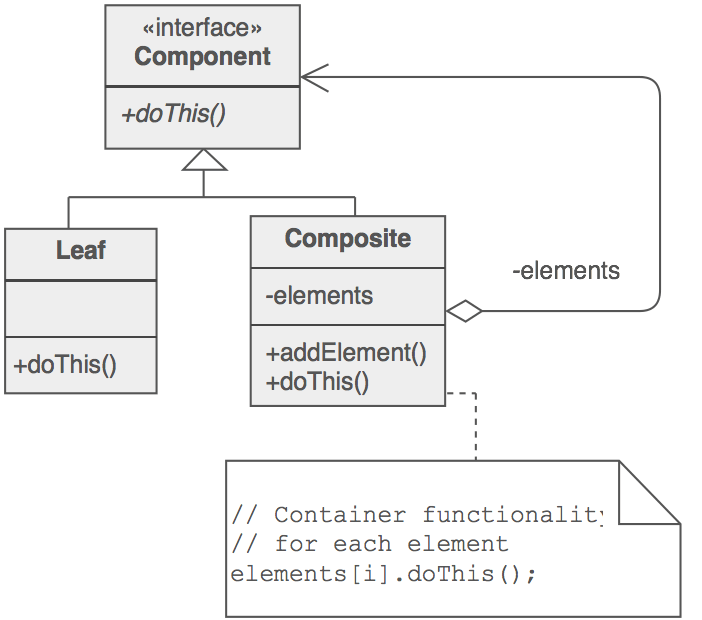
\includegraphics[width=200]{images/composite/UML.png}
    \caption{Estrutura exemplificativa do padrão \textit{Composite} em um diagrama de classes}
\end{figure}

\par Como é possível observar a partir da estrutra exemplificativa da Figura 1, existe a interface \textbf{\textit{Component}} (que poderia ser uma classe abstrata) onde estão definidos os métodos , o objeto composto (\textbf{\textit{Composite)}} e o objeto singular \textit{\textbf{(Leaf)}}. Independentemente do tipo de objeto, ambos implementam o mesmo método da interface, permitindo, no entanto,  a adição de outros objetos no objeto composto. Apesar do método ter o mesmo nome, dependendo do tipo do objeto, a implementação é diferente, sendo usual no objeto composto percorrer os filhos e chamar o mesmo método. \textbf{Todos os objetos são abordados de igual forma}.

\par Podem existir, no entanto, outros tipos de implementações ao utilizar este padrão com a possibilidade de permitir a remoção de objetos contidos no objeto composto ou, por exemplo, permitir apenas a substituição dos objetos guardados por novos, ao invés de adicionar, com o benefício da melhor compreensão do programa, mas reduzindo a flexibilidade. Dito isto, todas estas pequenas modificações sugeridas ao exemplo da Figura 1 continuam a manter a base do padrão \textit{Composite}, sendo totalmente válidas.

\clearpage
\subsection{Problema}

\par Tendo em conta o padrão de desenho de software \textit{Composite}, foi proposto um programa em Java que permite obter dados meteorológicos de aglomerados de localidades (distritos, vilas, etc.) bem como das localidades pertencentes a estes, e/ou apenas de localidades específicas. Os dados meteorológicos pretendidos são:
\begin{itemize}
    \item Tempo atual
    \item Temperatura atual
    \item Sumário da precipitação nas últimas 24 horas
\end{itemize}

\begin{figure}[!h]
    \centering
    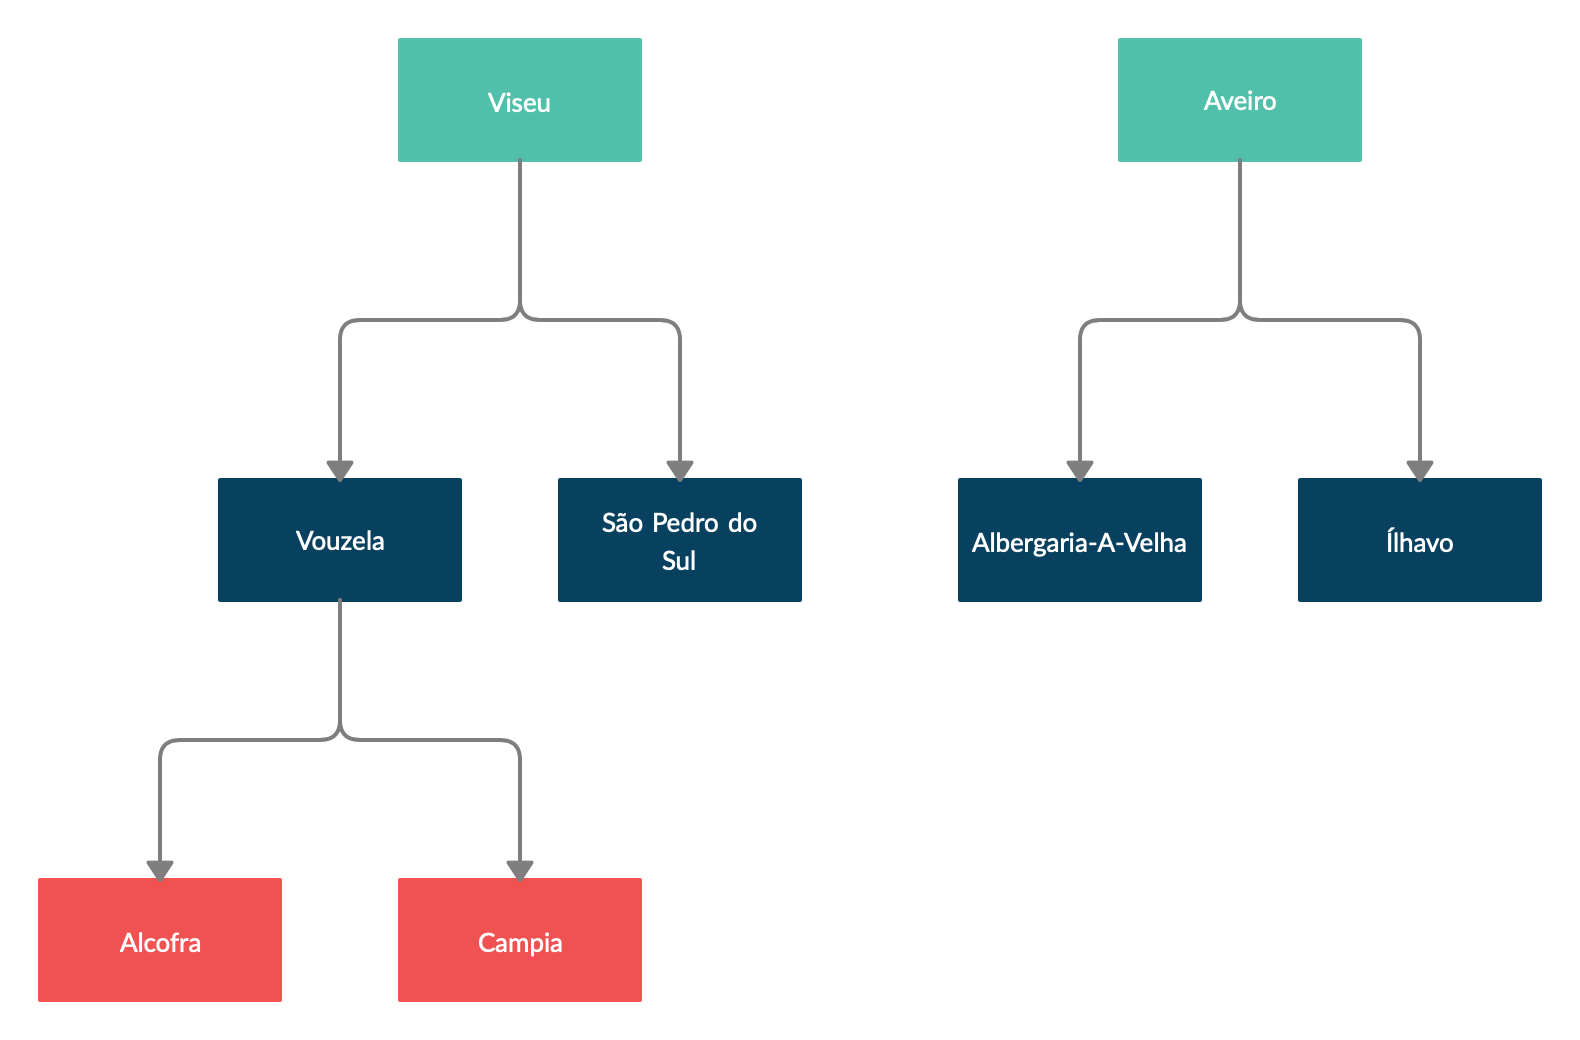
\includegraphics[width=325]{images/composite/tree.png}
    \caption{Exemplo de dados introduzidos na aplicação numa estrutura em árvore}
\end{figure}

\par Na Figura 2 é possível observar um exemplo de dados, associando, por exemplo, Viseu e Aveiro a localidades compostas e Alcofra e Campia a localidades singulares derivadas da localidade composta Vouzela. Ao introduzir os dados no programa este tem de ser capaz de lidar com cada localidade, independentemente do tipo e apresentar os dados meteorológicos da mesma. No caso de localidades compostas, é também necessário apresentar os dados das derivadas.

\clearpage

\subsection{Solução}

\par Sendo que a este problema pode ser aplicada uma estrutura em árvore com dois tipos de localidades (localidades compostas por outras e localidades singulares) e estas têm de ser tratadas de igual forma, fez sentido associar a sua resolução ao \textit{Composite}.

\begin{figure}[!h]
    \centering
    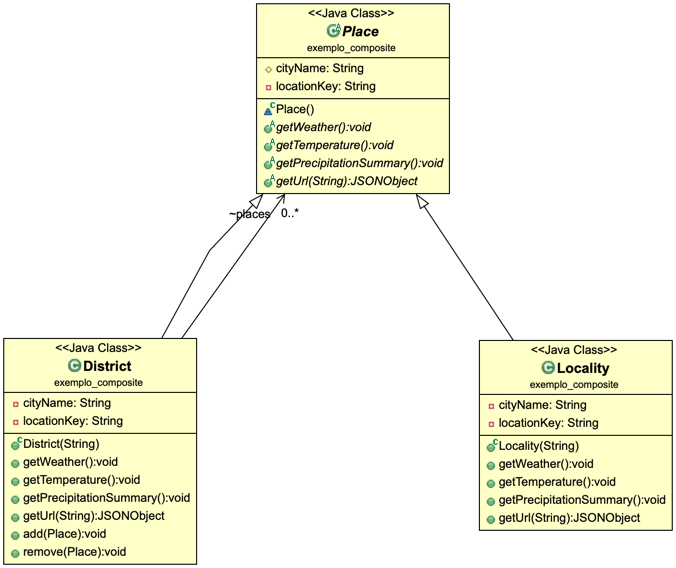
\includegraphics[width=300]{images/composite/UML_Example.png}
    \caption{Diagrama de classes da solução ao problema de exemplo do padrão \textit{Composite}}
\end{figure}

\par De acordo com o diagrama de classes (Figura 3) da solução apresentada, é possível observar a existência de duas classes representado os dois tipos de localidades. \textit{District} representa as localidade compostas e \textit{Locality} representa as localidades singulares. Ambas as classes extendem a classe abstrata \textit{Place} onde estão definidos os requisitos de todos os tipos de localidades, de maneira a serem tratadas de igual forma como dita o \textit{Composite}.

\par Foram utilizados como exemplo de dados desta solução, Lisboa, Aveiro e Amadora como localidades compostas e Reboleira, Alfragide, Sintra, Albergaria e Murtosa como localidades singulares. Reboleira e Alfragide fazem parte da Amadora, que por si só, faz parte de Lisboa. Albergaria e Murtosa fazem parte de Aveiro.

\subsubsection{\textit{Place}}

\par Seguindo a base do padrão, foi implementada uma classe abstrata que define os 4 métodos e 2 atributos, ambos necessários em todos os tipos de localidade e que permitem tratar os objetos da mesma forma:

\begin{itemize}
    \item \textbf{Atributo \textit{cityName}} - Guarda o nome da localidade
    \item \textbf{Atributo \textit{locationKey}} - Guarda o identificador correspondente à localidade, necessária para fazer chamadas à API AccuWeather
    \item \textbf{Método \textit{getWeather()}} - Responsável por obter o tempo atual
    \item \textbf{Método abstrato \textit{getTemperature()}} - Responsável por obter a temperatura atual
    \item \textbf{Método abstrato \textit{getPrecipitationSummary()}} - Responsável por obter sumário da precipitação nas últimas 24 horas
    \item \textbf{Método abstrato\textit{getUrl(String url)}} - Responsável por fazer chamadas à API, dependendo do pedido pretendido
\end{itemize}

\subsubsection{\textit{Locality}}

\par Extendendo a classe \textit{Place}, \textit{locality} implementa os métodos e atributos definidos pela sua classe superior.

\par A sua modelação permite ao cliente instanciá-la passando o nome da localidade que pretende obter os dados meteorológicos. Utilizando a API do serviço de meteorologia AccuWeather, é feito, na instanciação, um pedido para obter o identificador (\textit{key}) da localidade pretendida o qual é guardado no atributo \textit{locationKey}, juntamente com o nome da localidade no atributo \textit{cityName}, ambos definidos na classe superior.

\par Após a instanciação, qualquer um dos 3 métodos \textit{getWeather()}, \textit{getTemperature()} e \textit{getPrecipitationSummary()} podem ser utilizados para obter os dados, de acordo com a necessidade. Todos estes 3 métodos, bem como o construtor, utilizam o método \textit{getUrl(String url)} para fazer os pedidos à API, passando o url do pedido, interpretando posteriormente os dados recebido em JSON, através da livraria \textit{JSON.simple}. 

\subsubsection{\textit{District}}

\par Novamente, extendendo a classe \textit{Place}, \textit{District} é semelhante à classe \textit{Locality} nos métodos que implementam.

\par \textit{getWeather()}, \textit{getTemperature()} e \textit{getPrecipitationSummary()} funcionam da mesma forma que foi explicada anteriormente mas, visto estarem implementados numa classe que representa objetos compostos, ao invés de executar, apenas, as instruções para a sua localidade, invocam o mesmo método em todos os seus derivados, obtendo não só os dados metereológicos de si próprios, mas também dos seus filhos. 

\par Naturalmente, ao representar objetos compostos, são suportados dois novos métodos e um atributo:

\begin{itemize}
    \item \textbf{Atributo \textit{places}} - Guarda as várias localidades adicionadas
    \item \textbf{Método \textit{add(Place p)}} - Responsável por permitir a adição de novas localidades
    \item \textbf{Método abstrato \textit{remove(Place p)}} - Responsável por permitir a remoção de localidades
    
\end{itemize}



\clearpage

\section{Command}
\subsection{Descrição}

\par É expectável que um padrão de desenho de software comportamental, para além de fornecer boas práticas para resolver um determinado problema, foque as mesmas na forma como as classes e objetos interagem e distribuem responsabilidades.\textit{Command}, sendo um destes tipos de padrões, foca-se exactamente nesse ponto.

\par O problema que este padrão resolve incide não só na repetição de código mas também na organização geral das classes e das responsabilidades. \textbf{Separando o objeto que invoca uma ação do que a executa ao colocar um objeto intermediário, que implementa uma interface, o \textit{Command}, este intermediário é responsável por chamar o método que desempenha a ação no objeto receptor}.
Ao fazer isto, cada objeto tem a sua responsabilidade e são evitados os problemas de repetição de código pois, o objeto intermediário pode ser reutilizado múltiplas vezes, bem como problemas relacionados com limitações de comandos ou de alterações às outras entidades. Estes últimos dois são explicados devido ao facto de, ao utilizar objetos que implementam uma interface \textit{Command}, podemos não só criar novas classes de objetos que implementam esta interface com ações novas mas, também, alterar as outras entidades, desde que estas continuem a aceitar objetos que implementem a interface, sendo, portanto, um código mais flexível.

\par No fundo, \textbf{está-se a encapsular um pedido num objeto}, criando a possibilidade de adicionar mais métodos ao objeto criado, complementares à simples ação pedida pelo cliente.
A aproximação mais usual é a adição de um método que permite reverter o comando no entanto, o céu é o limite, é possível criar métodos que permitem adicionar um simples atraso à operação, até à execução de múltiplos comandos com apenas um pedido.


\begin{figure}[!h]
    \centering
    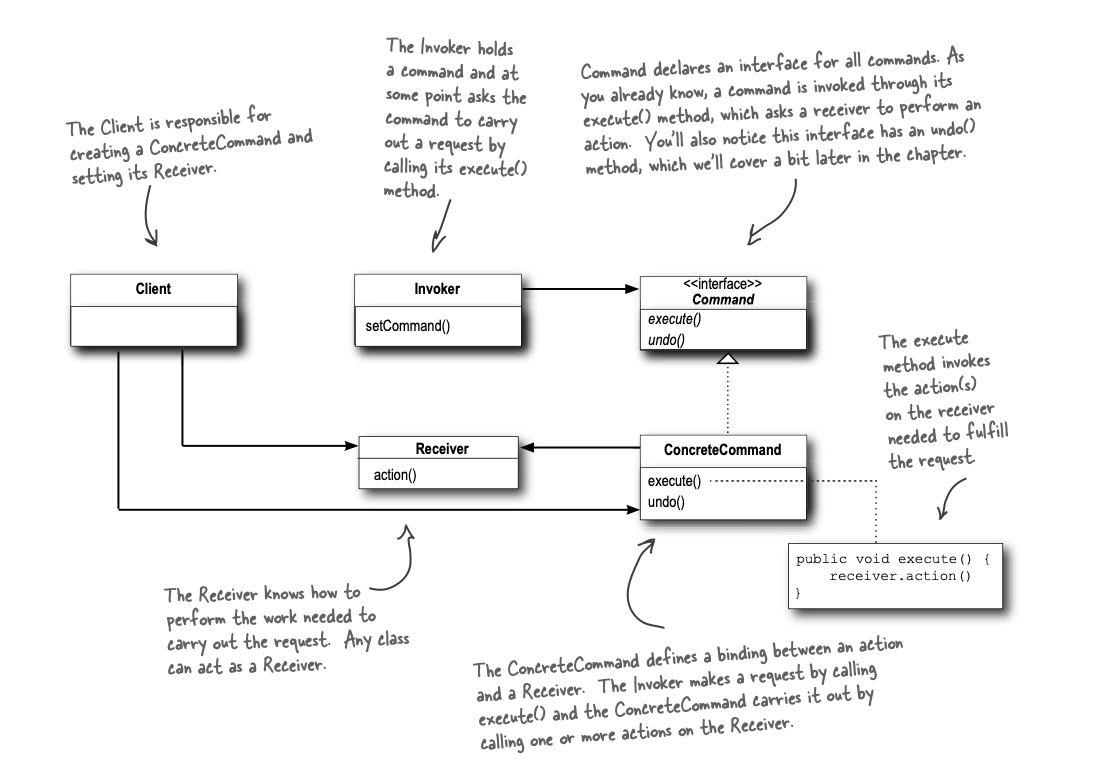
\includegraphics[width=415]{images/command/UML.png}
    \caption{Estrutura exemplificativa do padrão \textit{Command} em um diagrama de classes}
\end{figure}

\par Como é possível observar a partir da estrutura exemplificativa da Figura 4\footnote{}, a interface \textbf{\textit{Command}} onde estão definidos os métodos que os objetos representativos de uma ação irão implementar dita a possibilidade de executar uma dada ação ou reverté-la. Estes objetos estão a encapsular os pedidos do \textit{\textbf{Invoker}} e, posteriormente, invocam os métodos necessários para satisfazer o pedido no \textit{\textbf{Receiver}}. Visto que a interface suporta um método que desfaz a ação desse comando, o cliente pode utilizá-lo exatamente com esse fim, sendo que os objetos que representam uma ação têm de invocar os métodos necessários no \textit{\textbf{Receiver}} para concluir a reversão.

\par Considerando, por exemplo, um comando de televisão, este executa múltiplas ações sobre uma televisão, repetindo as ações ao longo da sua utilização. Aproximando este exemplo a uma linguagem de programação, não faria sentido, sempre que um determinado botão fosse clicado, criar um novo objeto com um determinado método ou até mesmo executar um código repetidamente, que apenas funcionaria para uma televisão em específico. 
Seguindo a lógica do \textit{Command}, faz muito mais sentido instanciar uma classe que armazena a televisão recetora do pedido e que, daí em diante, apenas necessita que lhe chamem o seu método específico para executar a ação, reutilizando e uniformizando o código. 

\par Um dos exemplo mais banais desta situação é toda a gestão que um programa ou sistema operativo faz dos \textit{inputs} de um utilizador. 
Ao utilizar, por exemplo, qualquer tipo de editor de texto, o sistema operativo permite ao utilizador inserir caracteres num campo mas, permite, também, reverter essas inserções (com a ajuda do atalho \textit{ctrl+z}). Ora, isto é um exemplo visível onde faria sentido aplicar este padrão de desenho de software.

\par Pessoalmente, sendo um utilizador casual de algum software de edição de imagens e vídeo (\textit{Adobe Photoshop, Adobe Illustrator e Final Cut Pro}), ao associar o \textit{Command} à gestão que estes programas fazem das ações dos utilizadores, os conceitos análogos ao mesmo tornaram-se ainda mais claros. Pegando no exemplo do \textit{Adobe Photoshop}, todas as alterações que são feitas a uma imagem podem ser desfeitas múltiplas vezes, tanto pela mesma ordem em que foram executadas, como também voltar a refazê-las, novamente, na ordem inversa. 
Ora, aproximando novamente a uma linguagem de programação, estas ações podem muito bem ser executadas com recurso ao padrão \textit{Command} ao encapsular os pedidos do utilizador em objetos. Estes objetos podem também ser introduzidos numa lista onde constam todos os pedidos recentes. 
Ao utilizar os famosos atalhos para desfazer e refazer (\textit{ctrl+z e ctrl+shift+z}), o programa apenas teria de utilizar o método para desfazer a ação e percorrer a lista na ordem inversa. O mesmo se aplica para refazer as ações desfeitas, sendo apenas necessário utilizar o método para executar a ação e percorrer novamente a lista já na ordem "normal".





\par Como em todos os padrões de desenho de software, a implementação mais correta é sempre discutível pois, apesar de uma solução se desviar da solução-base, esta pode ser justificada de acordo com o problema.

\clearpage

\subsection{Problema}

\par Foi proposta a criação de um labirinto em Java que, para além dos comandos normais de movimento, permita desfazer essas ações.

\begin{figure}[!h]
    \centering
    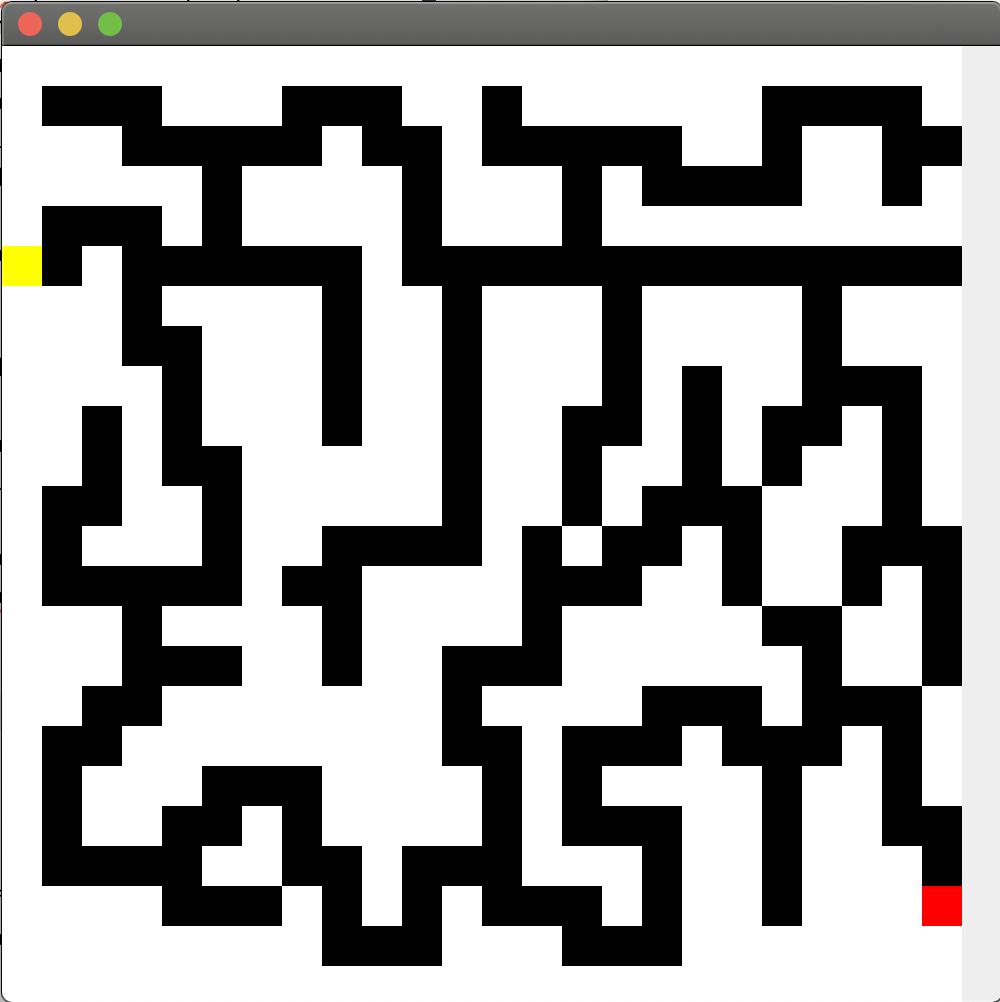
\includegraphics[width=325]{images/command/labirinto.png}
    \caption{Labirinto sugerido para a resolução desta proposta}
\end{figure}

\par Na Figura 2 é possível observar um exemplo de dados, associando, por exemplo, Viseu e Aveiro a localidades compostas e Alcofra e Campia a localidades singulares derivadas da localidade composta Vouzela. Ao introduzir os dados no programa este tem de ser capaz de lidar com cada localidade, independentemente do tipo e apresentar os dados meteorológicos da mesma. No caso de localidades compostas, é também necessário apresentar os dados das derivadas.


\subsection{Solução}

\begin{figure}[!h]
    \centering
    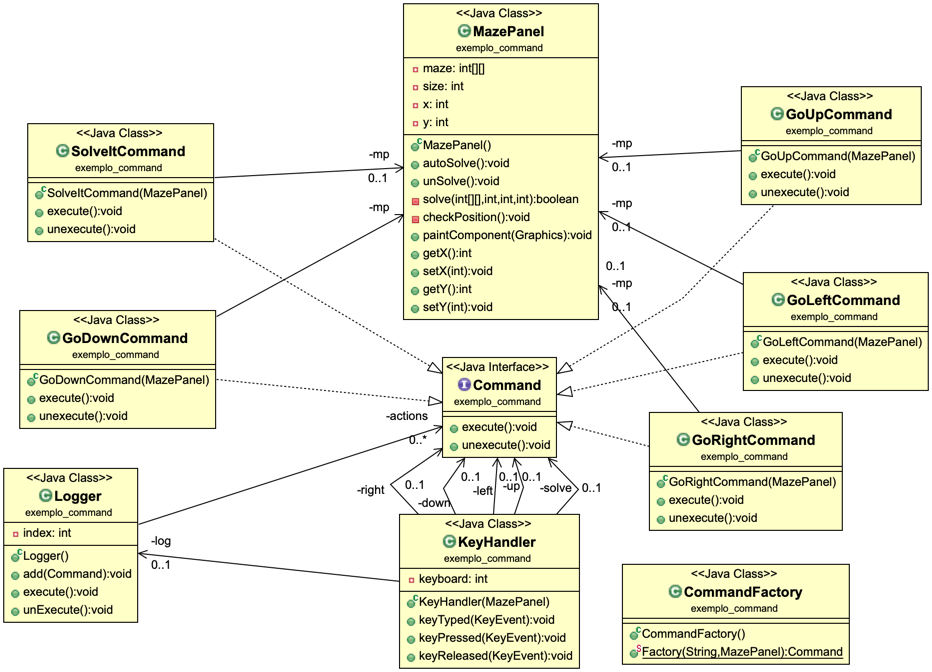
\includegraphics[width=325]{images/command/UML_Example.png}
    \caption{Diagrama de classes da solução apresentada ao problema de exemplo do padrão \textit{Command}}
\end{figure}


\clearpage

\section{Bibliografia}

\bibliographystyle{plain}

\bibliography{biblist}

\vspace{5mm} %5mm vertical space

\par \textbf{Composite:}

[1] \url{https://www.geeksforgeeks.org/composite-design-pattern/}

[2] \url{https://refactoring.guru/design-patterns/composite}

[3] \url{https://sourcemaking.com/design_patterns/composite}

[4] \url{https://www.tutorialspoint.com/design_pattern/composite_pattern.htm}

[5] \url{https://www.baeldung.com/java-composite-pattern}

[6] \url{https://developer.accuweather.com}

[7] \url{https://www.journaldev.com/7148/java-httpurlconnection-example-java-http-request-get-post}

[8] \url{http://miamarti.github.io/HorusFramework/javadoc/org/json/simple/parser/package-summary.html}

[9] \url{http://miamarti.github.io/HorusFramework/javadoc/org/json/simple/package-summary.html}


\par \textbf{Command:}

[1] \url{https://sourcemaking.com/design_patterns/command}

[2] \url{https://refactoring.guru/design-patterns/command}

[3] \url{https://www.tutorialspoint.com/design_pattern/command_pattern.htm}

[4] \url{https://www.geeksforgeeks.org/command-pattern/}

[5] \url{https://medium.com/better-programming/the-command-design-pattern-2313909122b5}

[6] \url{https://www.nku.edu/~foxr/CSC360/Programs/MazeWithGraphics.java}



\end{document}

